\documentclass[tikz]{standalone}\input{pre.tex}\begin{document}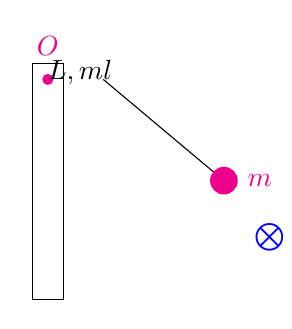
\begin{tikzpicture}


	\fill[magenta] (0,0) circle (2pt) node[above, yshift=0.5em] {$O$};

	\draw (0,0)++(-0.2,0.2) rectangle ++ (0.4,-3);
	\lineann[2]{90}{-2.8}{$L, m$}

	\draw (0,0) -- ++(-40:2) coordinate (g);

	\fill[magenta] (g) circle (5pt) node [right, xshift=0.5em] {$m$};
	\lineann[2]{-40}{2}{$l$}

	\draw (2,-2) node[blue] {$\bigotimes$} node[right, xshift=.5em] {$\vec{N}$};

\end{tikzpicture}\end{document}